% Dit werk is gelicenseerd onder de licentie Creative Commons Naamsvermelding-GelijkDelen 4.0 Internationaal. Ga naar http://creativecommons.org/licenses/by-sa/4.0/ om een kopie van de licentie te kunnen lezen.
\documentclass[t]{beamer}

\usepackage{amsmath,amsthm}             % Uitgebreide wiskundige mogelijkheden
\usepackage{xcolor}						% Om kleuren te gebruiken

%%%%%%%%%%%%%%%%%%%%%%%%%%%%%%%%%%%%%%%%%%%%%%%%%%%%%%%%%%%%
% Nieuwe commandos
%%%%%%%%%%%%%%%%%%%%%%%%%%%%%%%%%%%%%%%%%%%%%%%%%%%%%%%%%%%%

% De differentiaal operator
\newcommand{\diff}{\ensuremath{\mathrm{d}}}
\newcommand{\subsdiff}{\ensuremath{\mathrm{D}}}
\newcommand{\vardiff}{\ensuremath{\mathrm{\delta}}}

% Super en subscript
\newcommand{\supsc}[1]{\ensuremath{^{\text{#1}}}}   % Superscript in tekst
\newcommand{\subsc}[1]{\ensuremath{_{\text{#1}}}}   % Subscript in tekst

% Vectoren en matrices
\newcommand{\vt}[1]{\ensuremath{\boldsymbol{#1}}} % vector in juiste lettertype
\newcommand{\mx}[1]{\ensuremath{\mathsf{#1}}}	  % matrix in juiste lettertype

% Nieuw commando om iets te benadrukken en tegelijkertijd in de index te steken.
\newcommand{\begrip}[1]{\index{#1}\textbf{#1}\xspace}

% Graden celcius
\newcommand{\degC}{\ensuremath{^\circ \mathrm{C}}}
% graden
\renewcommand{\deg}{\ensuremath{^\circ}}

% unit
\newcommand{\unit}[1]{\ensuremath{\mathrm {#1}}}


% underlinered
\newcommand{\underlinered}[1]{\color{red}\underline{{\color{black}#1}}\color{black}}
%%%%%%%%%%%%%%%%%%%%%%%%%%%%%%
% Packages
%%%%%%%%%%%%%%%%%%%%%%%%%%%%%%

%\usepackage{geometry}              	% 
\usepackage[dutch]{babel}               % Voor nederlandstalige hyphenatie (woordsplitsing)
\uselanguage{dutch}
\languagepath{dutch}
\usepackage{amsmath,amsthm}             % Uitgebreide wiskundige mogelijkheden
\usepackage{url}                        % Om url's te verwerken
\usepackage{graphicx,subfigure}         % Om figuren te kunnen verwerken
\usepackage[utf8]{inputenc}             % Om niet ascii karakters rechtstreeks te kunnen typen
\usepackage[section]{placeins}			% Om ervoor te zorgen dat floats binnen dezelfde section blijven
\usepackage{multicol}
\usepackage[absolute,overlay]{textpos}

%%%%%%%%%%%%%%%%%%%%%%%%%%%%%%
% Layout
%%%%%%%%%%%%%%%%%%%%%%%%%%%%%%
\usetheme{Frankfurt}
\usefonttheme[onlymath]{serif}
\AtBeginSection[]
{
  \begin{frame}
    \frametitle{Inhoud}
    \tableofcontents[currentsection]
  \end{frame}
}

\setbeamertemplate{navigation symbols}{}
\setbeamertemplate{footline}[page number]

%%%%%%%%%%%%%%%%%%%%%%%%%%%%%%
% Title
%%%%%%%%%%%%%%%%%%%%%%%%%%%%%%
\title{Fluïdummechanica}
\author{Brecht Baeten\inst{1}}
\institute{
	\inst{1}%
  		KU Leuven, Technologie campus Diepenbeek,\\ e-mail: brecht.baeten@kuleuven.be
}
\date{\today}
%%%%%%%%%%%%%%%%%%%%%%%%%%%%%%
% Omgevingen
%%%%%%%%%%%%%%%%%%%%%%%%%%%%%%


\subtitle{Leidingstelsels}

\begin{document}

	\frame{\titlepage}
%%%%%%%%%%%%%%%%%%%%%%%%%%%%%%%%%%%%%%%%%%%%%%%%%%%%%%%%%%%%%%%%%%%%%%%%%%%
	\section{Inleiding}
	\begin{frame}
		\frametitle{Voorbeeld}
		\center
    	\includegraphics[height=0.8\textheight]{../fig/leidingstelsels/piping.jpg}\\
    	\footnotesize{Bron: http://hollandaptblog.com}
  	\end{frame}
%%%%%%%%%%%%%%%%%%%%%%%%%%%%%%%%%%%%%%%%%%%%%%%%%%%%%%%%%%%%%%%%%%%%%%%%%%%
  	\section{Mechanische energie}
  	\begin{frame}
		\frametitle{Bernoulli}
		\only<1-4>{
			Behoud van mechanisch energie:
			\begin{equation*}
				p_2 + \rho \frac{1}{2} v_2^2 + \rho g z_2 = p_1 + \rho \frac{1}{2} v_1^2 + \rho g z_1
			\end{equation*}
		}
		\only<2-4>{
			Door viskeuze wrijving wordt een gedeelte van de mechanische energie gedissipeerd:
			\begin{equation*}
				p_2 + \rho \frac{1}{2} v_2^2 + \rho g z_2 = p_1 + \rho \frac{1}{2} v_1^2 + \rho g z_1 - \Delta E
			\end{equation*}
		}
		\only<3-4>{
			Voor een rechte horizontale cilindrische leiding:
			\begin{equation*}
				\Delta E = p_1 - p_2  
			\end{equation*}	
		}
		\only<4-4>{
			\begin{equation*}
				\Delta E = f \frac{1}{2} \rho v^2 \frac{L}{D}
			\end{equation*}
		}
	\end{frame}
%%%%%%%%%%%%%%%%%%%%%%%%%%%%%%%%%%%%%%%%%%%%%%%%%%%%%%%%%%%%%%%%%%%%%%%%%%%
  	\begin{frame}
		\frametitle{Ladingsverlies}
		\only<1-3>{
			Stel de vergelijking voor mechanische energie voor in eenheid hoogte:
			\begin{equation}
				\frac{p_2}{\rho g} + \frac{v_2^2}{2 g} + z_2 = \frac{p_1}{\rho g} + \frac{v_1^2}{2 g} + z_1 - h_L
			\end{equation}
		}
		\only<2-3>{
			Ladingsverlies voor een cilindrische leiding:
			\begin{equation}
				h_\mathrm{L} = f \frac{v^2}{2 g} \frac{L}{D}
			\end{equation}
		}
		\only<3-3>{
			\begin{equation}
				h_\mathrm{L} = 8 f \frac{\dot{V}^2}{g \pi^2} \frac{L}{D^5}
			\end{equation}
		}
	\end{frame}
%%%%%%%%%%%%%%%%%%%%%%%%%%%%%%%%%%%%%%%%%%%%%%%%%%%%%%%%%%%%%%%%%%%%%%%%%%%
  	\begin{frame}
		\frametitle{Grafische voorstelling}
		\center
		\only<1>{
			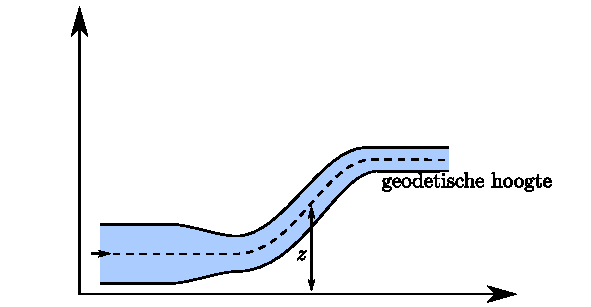
\includegraphics[width=\textwidth]{../fig/leidingstelsels/Energiehoogte0} \quad
		}
		\only<2>{
			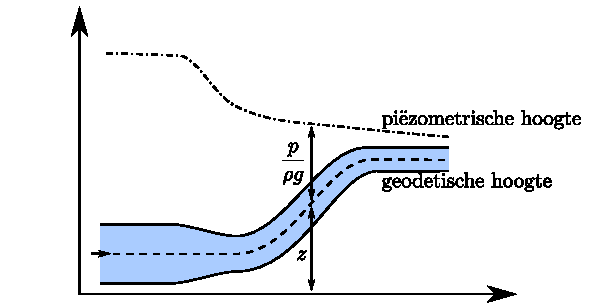
\includegraphics[width=\textwidth]{../fig/leidingstelsels/Energiehoogte1} \quad
		}	
		\only<3>{
			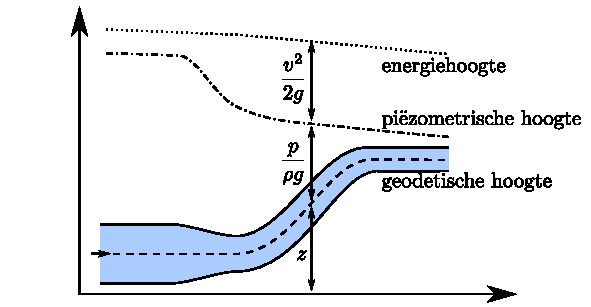
\includegraphics[width=\textwidth]{../fig/leidingstelsels/Energiehoogte2} \quad
		}	
		\only<4>{
			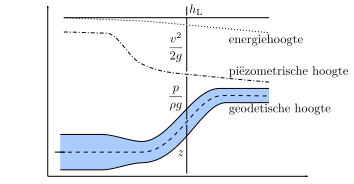
\includegraphics[width=\textwidth]{../fig/leidingstelsels/Energiehoogte} \quad
		}		
	\end{frame}
%%%%%%%%%%%%%%%%%%%%%%%%%%%%%%%%%%%%%%%%%%%%%%%%%%%%%%%%%%%%%%%%%%%%%%%%%%%
  	\section{Lokale ladingsverliezen}
  	\begin{frame}
		\frametitle{Voorbeelden}
		\center
		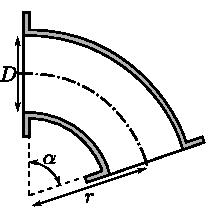
\includegraphics[width=0.3\textwidth]{../fig/appendix/Bocht} \quad
		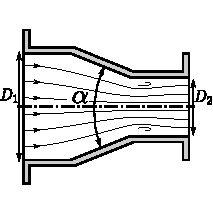
\includegraphics[width=0.3\textwidth]{../fig/appendix/Gelijdelijke_vernauwing} \quad
		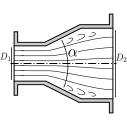
\includegraphics[width=0.3\textwidth]{../fig/appendix/Gelijdelijke_verwijding}
		\\
		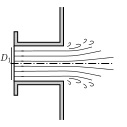
\includegraphics[width=0.3\textwidth]{../fig/appendix/Uitstroming} \quad
		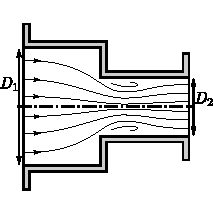
\includegraphics[width=0.3\textwidth]{../fig/appendix/Vernauwing} \quad
		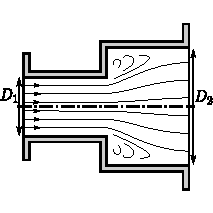
\includegraphics[width=0.3\textwidth]{../fig/appendix/Verwijding}
	\end{frame}
%%%%%%%%%%%%%%%%%%%%%%%%%%%%%%%%%%%%%%%%%%%%%%%%%%%%%%%%%%%%%%%%%%%%%%%%%%%
  	\begin{frame}
		\frametitle{Verliescoëfficient}	
		\only<1-3>{
			\center
			Lokale ladings verliezen kunnen in rekening gebracht worden met behulp van een empirisch bepaalde verliescoëfficient $\zeta$
		}
		
		\only<2-3>{
			\begin{equation*}
				h_\mathrm{L,lokaal} = \zeta \frac{v^2}{2 g}
			\end{equation*}
		}
		\only<3-3>{
			\begin{equation*}
				h_\mathrm{L,lokaal} = \zeta \frac{\dot{V}^2}{2 g A^2}
			\end{equation*}
		}
		
	\end{frame}
%%%%%%%%%%%%%%%%%%%%%%%%%%%%%%%%%%%%%%%%%%%%%%%%%%%%%%%%%%%%%%%%%%%%%%%%%%%
  	\begin{frame}
		\frametitle{Plotse Verwijding}
		\only<1>{
			\center
			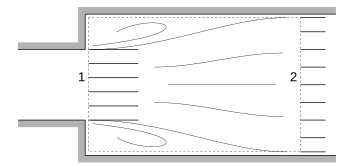
\includegraphics[width=\textwidth]{../fig/leidingstelsels/Plotse_verwijding}
		}
		\only<2-5>{
			\begin{textblock}{5}(0,3)
            	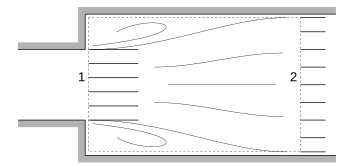
\includegraphics[width=5cm]{../fig/leidingstelsels/Plotse_verwijding}
       		\end{textblock}
       		\vspace{2.5cm}
		}
		\only<2-5>{
			\begin{equation*}
				p_1 A_2 - p_2 A_2 = \rho A_2 v_2 (v_2-v_1)
			\end{equation*}
		}
		\only<3-5>{
			\begin{equation*}
				\frac{p_2}{\rho g} + \frac{v_2^2}{2 g} = \frac{p_1}{\rho g} + \frac{v_1^2}{2 g} - h_L
			\end{equation*}
		}
		\only<4-5>{
			\begin{equation*}
				h_L = \frac{v_1^2}{2 g} \left(1 - 2\frac{v_2}{v_1} + \frac{v_2^2}{v_1^2} \right)
			\end{equation*}
		}
		\only<5-5>{
			\begin{equation*}
				h_L = \frac{v_1^2}{2 g} \left(1 - \frac{A_1}{A_2} \right)^2
			\end{equation*}
		}
	\end{frame}
%%%%%%%%%%%%%%%%%%%%%%%%%%%%%%%%%%%%%%%%%%%%%%%%%%%%%%%%%%%%%%%%%%%%%%%%%%%
  	\begin{frame}
		\frametitle{Voorbeeld van empirische data}
		\center
		\begin{tabular}{p{7cm} p{3cm}}
			\vtop{\null\hbox{
				\begin{tabular}{l c c c c c}
					$r/D$        & 1    & 2    & 4    & 6    & 10   \\
					\hline
					$\zeta$ glad & 0.21 & 0.14 & 0.11 & 0.09 & 0.11 \\
					$\zeta$ ruw  & 0.51 & 0.30 & 0.23 & 0.18 & 0.20 \\
				\end{tabular}
			}}
			&
			\vtop{\null\hbox{
				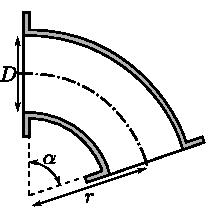
\includegraphics[width=3cm]{../fig/appendix/Bocht}
			}}
		\end{tabular}
		
		\center
		Het totale ladingsverlies is steeds het lokale verlies plus het verlies ten gevolge van de lengte van de leiding.
	
	\end{frame}
%%%%%%%%%%%%%%%%%%%%%%%%%%%%%%%%%%%%%%%%%%%%%%%%%%%%%%%%%%%%%%%%%%%%%%%%%%%	
	\begin{frame}
		\frametitle{Voorbeelden}
		\center
		\only<1>{
			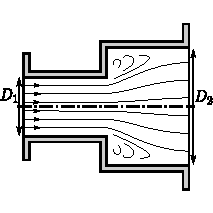
\includegraphics[height=0.8\textheight]{../fig/appendix/Verwijding}
		}
		\only<2>{
			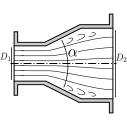
\includegraphics[height=0.8\textheight]{../fig/appendix/Gelijdelijke_verwijding}
		}
		\only<3>{
			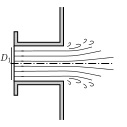
\includegraphics[height=0.8\textheight]{../fig/appendix/Uitstroming}
		}
		\only<4>{
			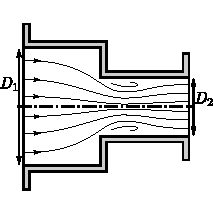
\includegraphics[height=0.8\textheight]{../fig/appendix/Vernauwing}
		}
		\only<5>{
			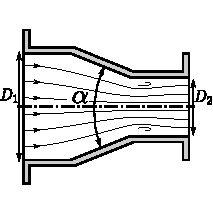
\includegraphics[height=0.8\textheight]{../fig/appendix/Gelijdelijke_vernauwing}
		}
		\only<6>{
			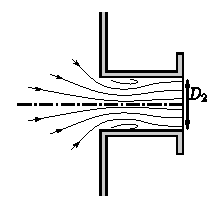
\includegraphics[height=0.8\textheight]{../fig/appendix/Instroming}
		}
		\only<7>{
			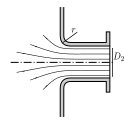
\includegraphics[height=0.8\textheight]{../fig/appendix/Afgeronde_instroming}
		}
	\end{frame}	
%%%%%%%%%%%%%%%%%%%%%%%%%%%%%%%%%%%%%%%%%%%%%%%%%%%%%%%%%%%%%%%%%%%%%%%%%%%
  	\section{Serie- en parallelschakeling}
  	\begin{frame}
		\frametitle{Serieschakeling}
		\only<1-3>{
			\center
			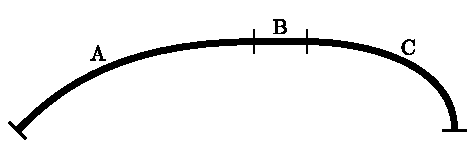
\includegraphics[width=0.8\textwidth]{../fig/leidingstelsels/serieschakeling}
		}
		\only<2-3>{	
			\begin{align*}
				\dot{V}_\mathrm{serie} &= \dot{V}_i \\
				h_\mathrm{L,serie} &= \sum h_{\mathrm{L},i}
			\end{align*}
		}
		\only<3-3>{
			\center
			Het totale ladingsverlies in een serieschakeling van elementen is de som van de ladingsverliezen
		}
	\end{frame}
%%%%%%%%%%%%%%%%%%%%%%%%%%%%%%%%%%%%%%%%%%%%%%%%%%%%%%%%%%%%%%%%%%%%%%%%%%%
  	\begin{frame}
		\frametitle{Parallelschakeling}
		\only<1-3>{
			\center
			\includegraphics[width=0.8\textwidth]{../fig/leidingstelsels/parallelschakeling}
		}
		\only<2-3>{	
			\begin{align*}
				\dot{V}_\mathrm{parallel} &= \sum \dot{V}_i \\
				h_\mathrm{L,parallel} &= h_{\mathrm{L},i}
			\end{align*}
		}
		\only<3-3>{
			\center
			Het ladingsverlies in elke tak van een parallelschakeling is gelijk aan het totale ladingsverlies
		}
	\end{frame}
%%%%%%%%%%%%%%%%%%%%%%%%%%%%%%%%%%%%%%%%%%%%%%%%%%%%%%%%%%%%%%%%%%%%%%%%%%%
  	\begin{frame}
  		\frametitle{Elektrisch analoog}
  		\only<1-4>{
  			\begin{equation*}
  				h_\mathrm{L} = 8 f \frac{\dot{V}^2}{g \pi^2} \frac{L}{D^5}
  			\end{equation*}
  		}
  		\only<2-4>{
  			\begin{equation*}
  				U = R I
  			\end{equation*}
  		}
  		\only<3-4>{
  			\begin{equation*}
  				h_\mathrm{L} = R \dot{V}^2
  			\end{equation*}
  		}
  		\only<4-4>{
  		
  			Voor leidingen:
  			\begin{equation*}
  				R = \frac{8 f}{g \pi^2} \frac{L}{D^5}
  			\end{equation*}
  			
  			Voor lokale verliezen:
  			\begin{equation*}
  				R = \frac{\zeta}{2 g A^2}
  			\end{equation*}
  		}
  		\only<5-6>{
  		
  			Serieschakeling:
  			\begin{align*}
  				h_\mathrm{L,serie} &= R_\mathrm{serie} \dot{V}^2\\
  				R_\mathrm{serie} &= \sum_i R_i 
  			\end{align*}
  		}
  		\only<6-6>{	
  		
  			Parallelschakeling:
  			\begin{align*}
  				h_\mathrm{L,parallel} &= R_\mathrm{parallel} \dot{V}^2\\
  				R_\mathrm{parallel} &= \left( \sum_i \frac{1}{\sqrt{R_i}} \right)^{-2}
  			\end{align*}
  		}
  	\end{frame}
%%%%%%%%%%%%%%%%%%%%%%%%%%%%%%%%%%%%%%%%%%%%%%%%%%%%%%%%%%%%%%%%%%%%%%%%%%%
  	\begin{frame}
  		\frametitle{Iteratief elektrisch analoog}
  		\only<1-4>{
  			\begin{equation*}
  				h_\mathrm{L} = 8 f \frac{\dot{V}^2}{g \pi^2} \frac{L}{D^5}
  			\end{equation*}
  		}
  		\only<2-4>{
  			\begin{equation*}
  				U = R I
  			\end{equation*}
  		}
  		\only<3-4>{
  			\begin{equation*}
  				h_\mathrm{L} = R' \dot{V}
  			\end{equation*}
  		}
  		\only<4-4>{
  		
  			Voor leidingen:
  			\begin{equation*}
  				R' = \frac{8 f}{g \pi^2} \frac{L}{D^5} \dot{V}
  			\end{equation*}
  			
  			Voor lokale verliezen:
  			\begin{equation*}
  				R' = \frac{\zeta}{2 g A^2} \dot{V}
  			\end{equation*}
  		}
  		\only<5-6>{
  		
  			Serieschakeling:
  			\begin{align*}
  				h_\mathrm{L,serie} &= R'_\mathrm{serie} \dot{V}\\
  				R'_\mathrm{serie} &= \sum_i R'_i 
  			\end{align*}
  		}
  		\only<6-6>{	
  		
  			Parallelschakeling:
  			\begin{align*}
  				h_\mathrm{L,parallel} &= R'_\mathrm{parallel} \dot{V}\\
  				R'_\mathrm{parallel} &= \left( \sum_i \frac{1}{R'_i} \right)^{-1}
  			\end{align*}
  		}
  		\only<7-8>{

  			\begin{equation*}
  				R' = \frac{8 f}{g \pi^2} \frac{L}{D^5} \underlinered{\dot{V}}
  			\end{equation*}
  			
  			Iteratieve oplossingsprocedure noodzakelijk
  			
  		}
  		\only<8-8>{
  			
  			\vspace{0.5cm}
  			\setbeamertemplate{enumerate items}[default]
			\begin{enumerate}
				\item Schat $\dot{V}_i$
				\item Bepaal $R'_i$
				\item Bepaal $\dot{V}_i$, en andere grootheden
				\item Indien de schatting te ver afwijkt van het resultaat: ga naar stap 2 
			\end{enumerate}  		
  		
  		}
  	\end{frame}
%%%%%%%%%%%%%%%%%%%%%%%%%%%%%%%%%%%%%%%%%%%%%%%%%%%%%%%%%%%%%%%%%%%%%%%%%%%
  	\begin{frame}
  		\frametitle{Voorbeeld}
		\only<1>{
			\center	
  			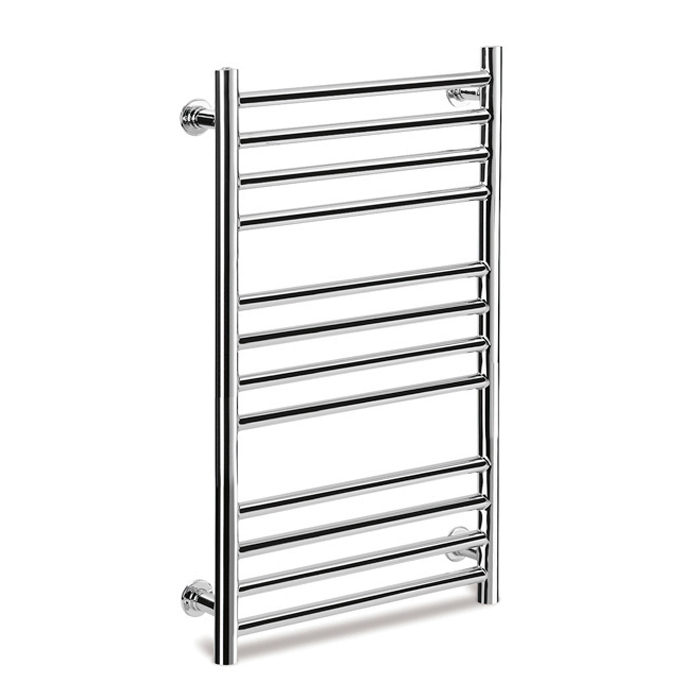
\includegraphics[height=0.8\textheight]{../fig/leidingstelsels/handdoekdroger.jpg}\\
            \footnotesize{Bron: http://www.aquaprestige.be}
  		}
  		\only<2-5>{
  			\begin{textblock}{5}(0,3)
        	    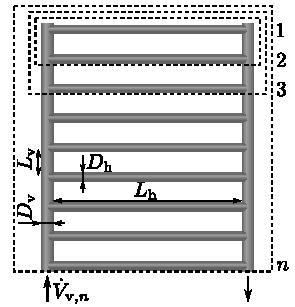
\includegraphics[width=4.5cm]{../fig/leidingstelsels/Handdoekdroger}
        	\end{textblock}
  		}
  		\begin{textblock}{6}(5.5,3)
  			\only<3-5>{
  				\begin{equation*}
  					h_{\mathrm{L},1\rightarrow 2} = \left( \frac{1}{\sqrt{R_{\mathrm{h},2}}} + \frac{1}{\sqrt{2R_{\mathrm{v},1}+R_{\mathrm{h},1}}} \right)^{-2} \dot{V}_{\mathrm{v},2}^2
  				\end{equation*}
  				\begin{equation*}
  					R_{1\rightarrow 2} = \left( \frac{1}{\sqrt{R_{\mathrm{h},1}}} + \frac{1}{\sqrt{2R_{\mathrm{v},1}+R_{\mathrm{h},1}}} \right)^{-2}
  				\end{equation*}
  			}
  			\only<4-5>{
  				\begin{equation*}
  					R_{1\rightarrow 3} = \left( \frac{1}{\sqrt{R_{\mathrm{h},3}}} + \frac{1}{\sqrt{2R_{\mathrm{v},2} + R_{1\rightarrow 2}}} \right)^{-2}
  				\end{equation*}
  			}
  			\only<5-5>{
  				\begin{align*}
  					R_{1\rightarrow n} &= \left( \frac{1}{\sqrt{R_{\mathrm{h},n}}} + \frac{1}{\sqrt{2R_{\mathrm{v},n-1}+R_{1\rightarrow n-1}}} \right)^{-2} \\
  					h_{\mathrm{L},1\rightarrow n} &= R_{1\rightarrow n} \dot{V}_{\mathrm{v},n}^2
  				\end{align*}
  			}
  			\only<6>{
  				code voorbeeld
  			}
  		\end{textblock}
  	\end{frame}
%%%%%%%%%%%%%%%%%%%%%%%%%%%%%%%%%%%%%%%%%%%%%%%%%%%%%%%%%%%%%%%%%%%%%%%%%%%
  	\begin{frame}
  		\frametitle{Voorbeeld iteratief}
  		\only<1-6>{
  			\begin{textblock}{5}(0,3)
        	    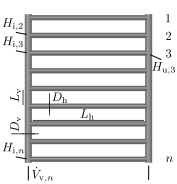
\includegraphics[width=4.5cm]{../fig/leidingstelsels/Handdoekdroger_iteratief}
        	\end{textblock}
  		}
  		\begin{textblock}{6}(6.0,3)
  			\only<2-3>{
  				\begin{equation*}
  					\frac{p_2}{\rho g} + \frac{v_2^2}{2 g} + z_2 = \frac{p_1}{\rho g} + \frac{v_1^2}{2 g} + z_1 - h_L
  				\end{equation*}
  			}
  			\only<3-3>{
  				\begin{equation*}
  					H_2 = H_1 - h_L
  				\end{equation*}
  			}
  			\only<4-5>{
  				\begin{align*}
  					H_{2,\mathrm{i}} &= H_{3,\mathrm{i}} - R'_{\mathrm{v},2} \dot{V}_{\mathrm{v},2} \\
  					H_{3,\mathrm{u}} &= H_{2,\mathrm{u}} - R'_{\mathrm{v},2} \dot{V}_{\mathrm{v},2} \\
  					H_{2,\mathrm{u}} &= H_{2,\mathrm{i}} - R'_{\mathrm{h},2} \dot{V}_{\mathrm{h},2}
  				\end{align*}
  			}
  			\only<5-5>{
				\begin{equation*}
  					\dot{V}_{\mathrm{h},2} = \dot{V}_{\mathrm{v},2} + \dot{V}_{\mathrm{h},1}
  				\end{equation*}
  			}
  			\only<6>{
  				\begin{align*}
  					H_{\mathrm{i},i} &= H_{\mathrm{i},i+1} - R'_{\mathrm{v},i} \dot{V}_{\mathrm{v},i} \\
  					H_{\mathrm{u},i+1} &= H_{\mathrm{u},i} - R'_{\mathrm{v},i} \dot{V}_{\mathrm{v},i} \\
  					H_{\mathrm{u},i} &= H_{\mathrm{i},i} - R'_{\mathrm{h},i} \dot{V}_{\mathrm{h},i} 
  				\end{align*}
				\begin{equation*}
  					\dot{V}_{\mathrm{h},i+1} = \dot{V}_{\mathrm{v},i+1} + \dot{V}_{\mathrm{h},i}
  				\end{equation*}
  			}
  		\end{textblock}
  		
		\only<7>{
  			
  			\vspace{-0.2cm}
  			\begin{equation*}
				\begin{pmatrix}
    &        &        &        &        &        &        &                   &        & \\
  0 & 1      & -1     & 0      &        &        &        & R'_{\mathrm{v},i} &        & \\
    & \ddots & \ddots & \ddots & \ddots &        &        &                   & \ddots & \\
    &        &        & 0      & -1     & 1      & 0      & R'_{\mathrm{v},i} &        & \\
    &        &        &        & \ddots & \ddots & \ddots & \ddots            & \ddots & \\
    &        &        &        &        &        &        &                   &        & \\
    &        &        &        &        & \vdots &        &                   &        & \\
\end{pmatrix}%
 \cdot
 \begin{pmatrix}
  \vdots \\
  H_{\mathrm{i},i} \\
  H_{\mathrm{i},i+1} \\
  \vdots \\
  H_{\mathrm{u},i} \\
  H_{\mathrm{u},i+1} \\
  \vdots \\
  \dot{V}_{\mathrm{v},i} \\
  \dot{V}_{\mathrm{v},i+1} \\
  \vdots \\
  \dot{V}_{\mathrm{h},i} \\
  \dot{V}_{\mathrm{h},i+1} \\
  \vdots
 \end{pmatrix}
 =
 \begin{pmatrix}
  \vdots \\
  0 \\
  \vdots \\
  0 \\
  \vdots \\
  \vdots \\
  \vdots \\
  0 \\
  \vdots \\
  \vdots \\
  0 \\
  \vdots
 \end{pmatrix}
  			\end{equation*}
  		}
  	\end{frame}
%%%%%%%%%%%%%%%%%%%%%%%%%%%%%%%%%%%%%%%%%%%%%%%%%%%%%%%%%%%%%%%%%%%%%%%%%%%
  	\begin{frame}
  		\frametitle{Toepassingen}
  		\begin{itemize}
  			\only<1,2-3>{
  				\item Bepaal het ladingsverlies
  			}
  			\only<1,4>{
  				\item Bepaal het debiet
  			}
  			\only<1,5>{
  				\item Bepaal de leiding diameter
  			}
  		\end{itemize}
  		\vspace{0.4cm}
  		
  		\only<2-3>{
  			Gegeven:\\
  			\qquad $\dot{V}, L, D,\varepsilon$

  			
  			Gevraagd:\\
  			\qquad $h_\mathrm{L}$	
  		}
  		\only<2>{
  		
  			\vspace{0.4cm}
  			Oplossingsmethode voor een serieschakeling van leidingen of een parallelschakeling van gelijke leidingen:
  			\setbeamertemplate{enumerate items}[default]
  			\begin{enumerate}
  				\item Bepaal $\mathrm{Re}$
  				\item Bepaal $f$
  				\item Bepaal $h_\mathrm{L}$
  			\end{enumerate}
  		}
  		\only<3>{
  		
  			\vspace{0.4cm}
  			Oplossingsmethode een parallelschakeling:
  			\setbeamertemplate{enumerate items}[default]
  			\begin{enumerate}
  				\item Schat $\dot{V}_i$
  				\item Bepaal $\mathrm{Re}_i$
  				\item Bepaal $f_i$
  				\item Bepaal $h_\mathrm{L}$
  				\item Bepaal $\dot{V}_i$
  				\item Ga naar stap 2
  			\end{enumerate}
  		}
		\only<4>{
  			Gegeven:\\
  			\qquad $h_\mathrm{L}, L, D,\varepsilon$

  			Gevraagd:\\
  			\qquad $\dot{V}$
  			
  			\vspace{0.4cm}
  			Oplossingsmethode:
  			\setbeamertemplate{enumerate items}[default]
  			\begin{enumerate}
  				\item Schat $\dot{V}$
  				\item Bepaal $\mathrm{Re}$
  				\item Bepaal $f$
  				\item Bepaal $\dot{V}$
  				\item Ga naar stap 2
  			\end{enumerate}
  		}
  		\only<5>{
  			Gegeven:\\
  			\qquad $\dot{V}, h_\mathrm{L}, L,\varepsilon$

  			Gevraagd:\\
  			\qquad $D$
  			
  			\vspace{0.4cm}
  			Oplossingsmethode:
  			\setbeamertemplate{enumerate items}[default]
  			\begin{enumerate}
  				\item Schat $D$
  				\item Bepaal $\mathrm{Re}$
  				\item Bepaal $f$
  				\item Bepaal $D$
  				\item Ga naar stap 2
  			\end{enumerate}
  		}
  	\end{frame}
%%%%%%%%%%%%%%%%%%%%%%%%%%%%%%%%%%%%%%%%%%%%%%%%%%%%%%%%%%%%%%%%%%%%%%%%%%%
  	\begin{frame}
  		\frametitle{Leidingnetwerk}
  		\only<1>{
  			\center
			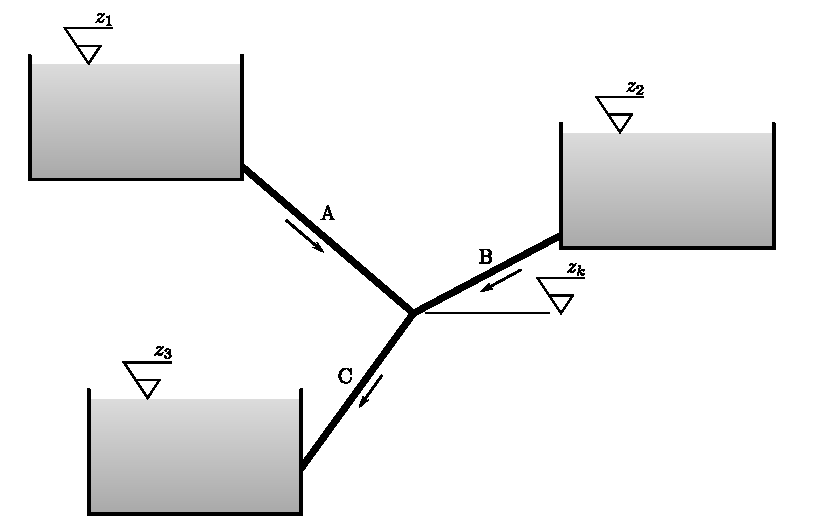
\includegraphics[width=\textwidth]{../fig/leidingstelsels/Leidingnetwerk}
		}
		\only<2-3>{
			\begin{textblock}{5}(0,3)
        	    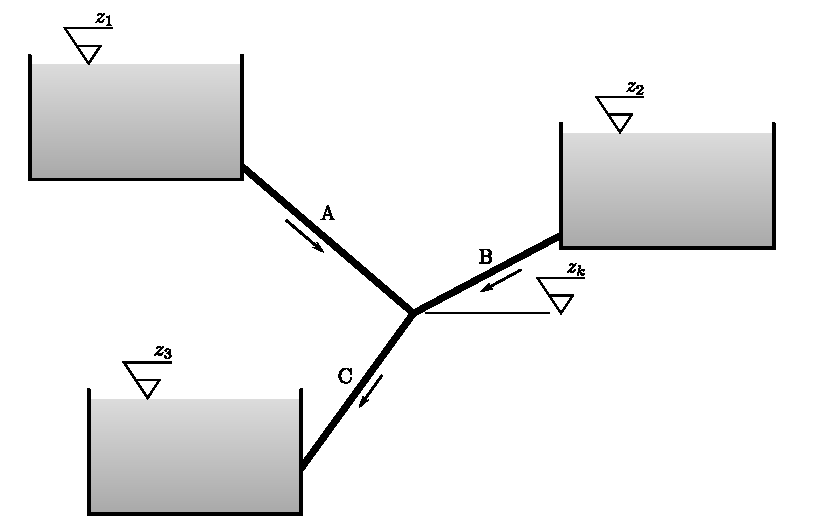
\includegraphics[width=5cm]{../fig/leidingstelsels/Leidingnetwerk}
        	\end{textblock}
        	\vspace{3cm}
  		}
  		\only<2>{
  			\begin{equation*}
				\left\{
					\begin{array}{lcl}
						h_k &=& \dfrac{p_1}{\rho g} + z_1 - h_{L,1} \\
						h_k &=& \dfrac{p_2}{\rho g} + z_2 - h_{L,2} \\
						\dfrac{p_3}{\rho g} + z_3 &=& h_k - h_{L,3} 
					\end{array}
				\right.
			\end{equation*}
		}
		\only<3>{
  			\begin{equation*}
				\left\{
					\begin{array}{lcl}
						h_k &=& \dfrac{p_1}{\rho g} + z_1 - h_{L,1} \\
						h_k &=& \dfrac{p_2}{\rho g} + z_2 - h_{L,2} \\
						\dfrac{p_3}{\rho g} + z_3 &=& h_k - h_{L,3} \\
						\dot{V}_3 &=& \dot{V}_1 + \dot{V}_2
					\end{array}
				\right.
			\end{equation*}
		}
    \end{frame} 
%%%%%%%%%%%%%%%%%%%%%%%%%%%%%%%%%%%%%%%%%%%%%%%%%%%%%%%%%%%%%%%%%%%%%%%%%%%
	\section{Pompen en ventilatoren}
  	\begin{frame}
  		\frametitle{Mechanische energie}
  		\only<1-4>{
  			\center
  			\textbf{Een pomp of ventilator voegt mechanische energie toe aan de stroming}
  		}
  		\only<2-4>{
  			\begin{equation*}
				\frac{p_2}{\rho g} + \frac{v_2^2}{2 g} + z_2 = \frac{p_1}{\rho g} + \frac{v_1^2}{2 g} + z_1 - h_\mathrm{L} + h_\mathrm{P}
			\end{equation*}
			Met $h_\mathrm{P}$ de opvoerhoogte.
  		}
  		\only<3-4>{
  			
  			\vspace{1cm}
  			\center
  			\textbf{Een turbine onttrekt mechanische energie aan de stroming}
  		}
  		\only<4-4>{
  			\begin{equation*}
				\frac{p_2}{\rho g} + \frac{v_2^2}{2 g} + z_2 = \frac{p_1}{\rho g} + \frac{v_1^2}{2 g} + z_1 - h_\mathrm{L} + h_\mathrm{P} - h_\mathrm{T}
			\end{equation*}
  		}
    \end{frame}
%%%%%%%%%%%%%%%%%%%%%%%%%%%%%%%%%%%%%%%%%%%%%%%%%%%%%%%%%%%%%%%%%%%%%%%%%%%   
  	\begin{frame}
  		\frametitle{Pomp- of ventilatorkarakteristiek}
  		\center
  		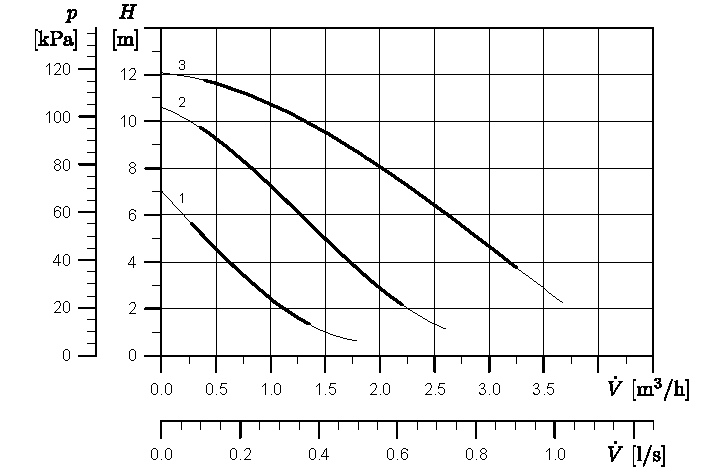
\includegraphics[width=\textwidth]{../fig/leidingstelsels/Pompkarakteristiek_UPS_25_120}
    \end{frame}
%%%%%%%%%%%%%%%%%%%%%%%%%%%%%%%%%%%%%%%%%%%%%%%%%%%%%%%%%%%%%%%%%%%%%%%%%%%   
  	\begin{frame}
  		\frametitle{Types pompen}
  		\center
  		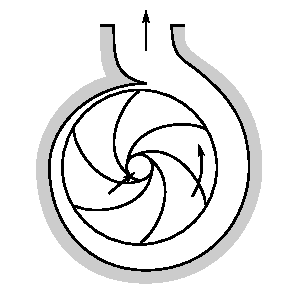
\includegraphics[width=0.3\textwidth]{../fig/leidingstelsels/Centrifugaalpomp}
  		\hspace{2cm}
  		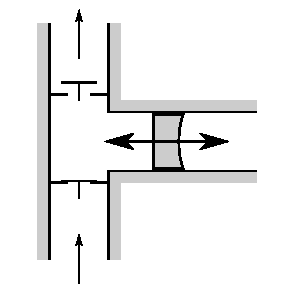
\includegraphics[width=0.3\textwidth]{../fig/leidingstelsels/Zuigerpomp}
  		
  		\vspace{0.5cm}
  		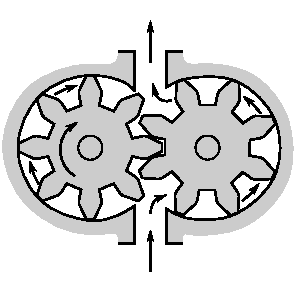
\includegraphics[width=0.3\textwidth]{../fig/leidingstelsels/Tandradpomp}
  		\hspace{2cm}
  		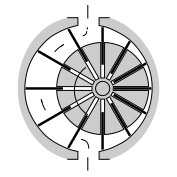
\includegraphics[width=0.3\textwidth]{../fig/leidingstelsels/Schottenpomp}
    \end{frame} 
%%%%%%%%%%%%%%%%%%%%%%%%%%%%%%%%%%%%%%%%%%%%%%%%%%%%%%%%%%%%%%%%%%%%%%%%%%% 
  	\begin{frame}
  		\frametitle{Leidingkarakteristiek}
  		\only<1>{
  			\begin{center}
  				\includegraphics{../fig/leidingstelsels/Leidingstelsel_pomp}
  			\end{center}
  		}
  		\only<2-3>{
  			\vspace{-0.6cm}
  			\begin{center}
  				\includegraphics[height=3cm]{../fig/leidingstelsels/Leidingstelsel_pomp}
  			\end{center}
  			
  			Het ladingsverlies plus het verschil in energiehoogte tussen uit- en inlaat is een functie van het debiet:
  			\begin{equation*}
  				h_\mathrm{L}(\dot{V}) + \left( \frac{p_2}{\rho g} + 8 \frac{\dot{V}^2}{g \pi^2 D_2^4} + z_2 \right) - \left( \frac{p_1}{\rho g} + 8 \frac{\dot{V}^2}{g \pi^2 D_1^4} + z_1 \right)
  			\end{equation*}
  		}
  		\only<3>{
  			\begin{equation*}
  				\frac{p_2}{\rho g} - \frac{p_1}{\rho g} + z_2 - z_1 + 8 \frac{\dot{V}^2}{g \pi^2 D_2^4} - 8 \frac{\dot{V}^2}{g \pi^2 D_1^4} + h_\mathrm{L}(\dot{V})
  			\end{equation*}
  		}
  		\only<4>{
  			\center
  			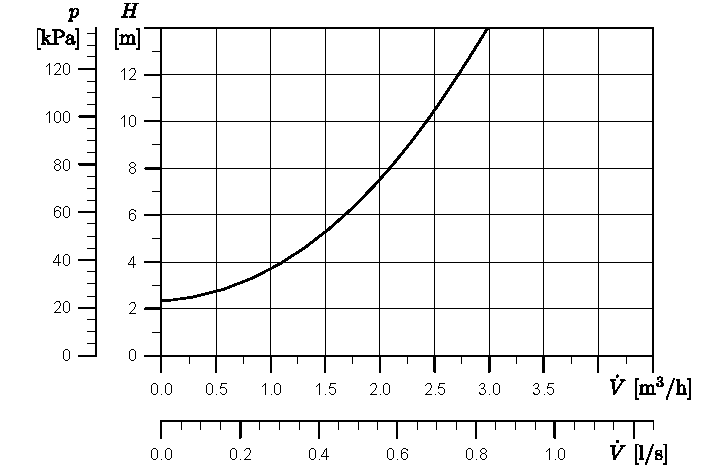
\includegraphics[width=\textwidth]{../fig/leidingstelsels/Leidingskarakteristiek}
  		}
    \end{frame}
%%%%%%%%%%%%%%%%%%%%%%%%%%%%%%%%%%%%%%%%%%%%%%%%%%%%%%%%%%%%%%%%%%%%%%%%%%% 
  	\begin{frame}
  		\frametitle{Werkingspunt}
  		\only<1>{
  			\center
  			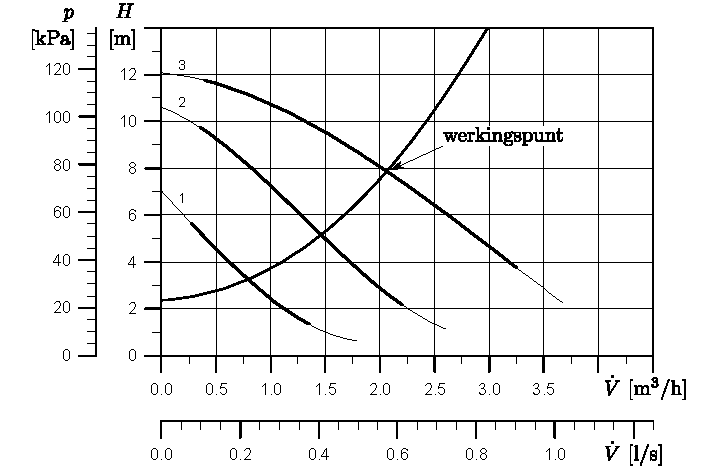
\includegraphics[width=\textwidth]{../fig/leidingstelsels/Pompleidingkarakteristiek}
  		}
  		\only<2-3>{
  			\center
  			\textbf{Het werkingspunt is het snijpunt van de pomp- en leidingkaraketeristiek}
  			
  			\begin{equation*}
  				h_\mathrm{L}(\dot{V}) + \left( \frac{p_2}{\rho g} + 8 \frac{\dot{V}^2}{g \pi^2 D_2^4} + z_2 \right) - \left( \frac{p_1}{\rho g} + 8 \frac{\dot{V}^2}{g \pi^2 D_1^4} + z_1 \right) = h_\mathrm{P}(\dot{V})
  			\end{equation*}
  		}
  		\only<3-3>{
  			\begin{equation*}
  				\frac{p_2}{\rho g} + 8 \frac{\dot{V}^2}{g \pi^2 D_2^4} + z_2  = \frac{p_1}{\rho g} + 8 \frac{\dot{V}^2}{g \pi^2 D_1^4} + z_1 - h_\mathrm{L}(\dot{V}) + h_\mathrm{P}(\dot{V})
  			\end{equation*}
  		}
    \end{frame} 
%%%%%%%%%%%%%%%%%%%%%%%%%%%%%%%%%%%%%%%%%%%%%%%%%%%%%%%%%%%%%%%%%%%%%%%%%%% 
  	\begin{frame}
  		\frametitle{Grafische voorstelling}
  		\only<1>{
  			\vspace{0.6cm}
  			
  			\center
			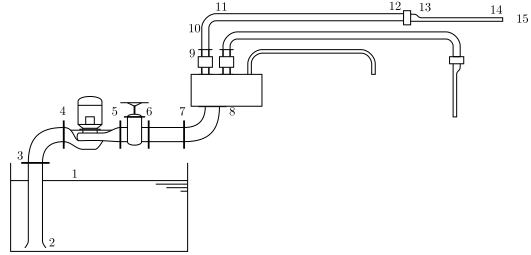
\includegraphics[width=\textwidth]{../fig/leidingstelsels/leiding_structuur}
		}
  		\only<2>{
  			\vspace{0.6cm}
  			
  			\center
			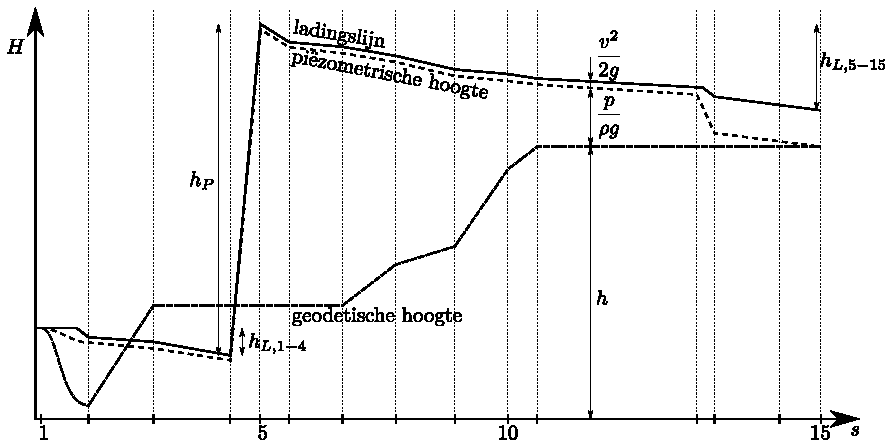
\includegraphics[width=\textwidth]{../fig/leidingstelsels/leidingstelsel_energiehoogte}
		}
    \end{frame} 
%%%%%%%%%%%%%%%%%%%%%%%%%%%%%%%%%%%%%%%%%%%%%%%%%%%%%%%%%%%%%%%%%%%%%%%%%%%
\end{document}